%---------DO NOT EDIT THIS INDENTED SECTION, EXCEPT TO ENTER YOUR NAME
	% Preamble
	\documentclass[11pt,reqno,oneside,a4paper]{article}
	\usepackage[a4paper,includeheadfoot,left=35mm,right=35mm,top=00mm,bottom=30mm,headheight=40mm]{geometry} %sets up the margins
	\usepackage{amssymb,amsmath,amsthm}
	\usepackage{xcolor,graphicx}
	\graphicspath{ {./capresults/} }
	\usepackage{verbatim}
	\usepackage{hyperref}
	\usepackage{titling}
	\usepackage{fancyhdr}
	\usepackage{natbib}
	\usepackage{tikz}
	\usepackage{booktabs}
	\usepackage{colortbl}
	\usepackage{rotating}
	\usepackage{threeparttable}
	\usepackage{longtable}
	\usepackage[nottoc]{tocbibind}
	\usepackage{setspace}
	\usepackage{pdfpages}
	\pagestyle{fancy} \lhead{{\theauthor}} \chead{} \rhead{} \lfoot{} \cfoot{\thepage} \rfoot{}
	%---The following code defines the title, author, and date of the document.
	\title{US Influence via Regime Change on Long-Run Inequality}
	\author{Alexander Christopher Horne}
	\date{\today}   % Using \today automatically updates to the document's build date
%----------------------------------

\doublespacing

\begin{document}

\includepdf{capstoneTitle}
\includepdf{declaration_and_consent_capstone_signed}

\maketitle
\thispagestyle{fancy}

%-----------EDIT FROM HERE

\begin{quote}
\textit{Using a country and year fixed effects model, I examine the effects of covert US interventions to install or support a foreign regime on within-country economic inequality over time. I find that successful interventions at regime change are associated with increases in measures of the Gini coefficient and top ten percent share of income or consumption, and this effect lasts up to 25 years following the intervention.}
\end{quote}

\tableofcontents{}

\section*{Acknowledgements}
\par{As much as this project has been self-directed, I am far from what the economics textbooks might call an independent, rational, and self-interested actor. Rather, I am made up of all those who have supported and nurtured me along the way. You could call me a community-made, emotional, and collective-interested actor.}
\par{This project has been a significant challenge to overcome, in no small part because at times I felt the need to drift away from all those who have supported me for so long in order to get done what needs getting done. The inner voice that I could never produce anything of value was particularly challenging to overcome.}
\par{The process was non-linear and often rocky, and I deeply appreciate everyone who quietly cheered me on and let me know that they were always there if I needed any help. While this paper is a mere slice in space and time, you all are what constitute life and what it means to \emph{live}. Thank you, in particular, to Claire, Scott, Tomas, Sam, Atharv, Manraaj, Sanat, and my family in (the suburbs of) Chicago and Kharkiv for being my bedrock of care and support, and for believing in me. Thank you, thank you, thank you.}

%%%%%%%%%%%%%%%% INTRO %%%%%%%%%%%%%%%%%%%%
\section{Introduction}

\par{Inequality has been the subject of much political, economic, and moral concern, and with recent improvements in data collection capability, economic inequality and its causes can be studied with more accuracy. In the words of Atkinston, ``if we are concerned about equality of opportunity tomorrow, we need to be concerned about inequality of outcome today." Recent studies have focused on the impact of finance on inequality \citep{de2017finance}, while others have focused on more macro-level factors that drive inequality such as education, technology, tax policy, and social norms regarding equality \citet{piketty2014inequality}.}
\par{A particularly important relationship is that of economic growth and inequality. While the popular mantra ``Growing the Pie" implies more growth means more for everyone, \citet{ravallion2004pro} found that improvements in poverty respond slower to economic growth when income inequality is high. In the other direction, the OECD has found that increasing income inequality has impeded economic growth, with high-inequality countries exhibiting low levels of social mobility due to limited access of the poor to quality education \citep{oecd2015together}.}
\par{The United States and its foreign policy have also been a matter of popular debate and scrutiny, particularly following its regular involvement in regime change during and after the Cold War. However, classification of CIA (Central Intelligence Agency) documents have often been an impediment to studying the effects of covert CIA interventions. Cold War documents, though, have now been mostly declassified, and \citet{berger2013superpower} created a time series cross sectional dataset that allows for the examination of the effects of successful US covert interventions to install or support a regime on any outcome variable of interest. This variable will be further discussed in the Data section; however, it is important to note that it encodes only \emph{successful} interventions in regime change or support, which is an essential aspect of both \citet{berger2013superpower}, \citet{berger2013commercial}, and my own mechanism.}
\par{I am interested in answering the question of whether US interventions and influence over a regime have an effect on economic inequality, and if so, what is the duration and magnitude of this effect?}
\par{My particular concern is with the long-run outcomes of income inequality in the aftermath of US interventions rather than the causes or goals of the interventions, however, the drivers of US interventions are of interest insofar as they introduce potential sources of endogeneity (or instruments). \citet{mullenbach2008deciding} find that several factors that significantly drive the likelihood of a US intervention, including geographic proximity, ethnic linkage (i.e., if there exists an ethnic group in the US that aligns with a minority ethnic group in the target country), humanitarian linkage (i.e., if there are many civilian fatalities or displaced civilians), and democracy. While I control for democracy in my analysis, the other variables are not included because they have no apparent effect on \emph{covert} CIA interventions as well as long-run inequality outcomes. As for domestic variables that could potentially serve as instruments, \citet{mullenbach2008deciding} find no evidence for any domestic factors consistently significantly driving the likelihood of US interventions. \citet{aubone2013explaining} summarizes much of the literature regarding drivers of US interventions and finds that the US has a lower likelihood of intervention when the target country has greater resource wealth and economic development. This introduces a potential source of selection bias which I address through both a log GDP per capita control variable and country and year fixed effects. In addition, as there may be certain time- and country-covarying omitted factors, I include a lagged dependent variable to control for pre-trends in inequality.}
\par{The question of US interventions and its effect on economic outcomes is particularly interesting in its ability to answer to what extent an outside great power can influence a regime, its policies, institutions, and real long-run social and economic dynamics.}




%%%%%%%%%%%%%%%% LIT REVIEW %%%%%%%%%%%%%%%%%%%%
\section{Related literature}

\par{This paper is most closely related to \citet{berger2013superpower} and \citet{berger2013commercial}, evaluating the effects of covert CIA interventions on outcomes in the target foreign countries. Those two papers found, respectively, that covert CIA interventions are associated with a significant decline in democracy and a larger share of imports from the US relative to total exports. In the same vein of US imperialism, a large body of literature has been written on the institutional and conflict-related effects of US interventions and aid \citep{nunn2014us} \citep{dube2015bases}\citep{magesan2018out}.}

\par{Older literature that has studied the effects of US military interventions on democracy have found no effect \citep{meernik1996united}, a positive effect \citep{hermann1998us}, or a positive effect when the intervention supports ``free and fair" elections \citep{peceny1999forcing}. While these papers included some controls, they suffered from a lack of available data and sufficient control variables. This is evident in the further research done on the topic, such as by \citet{bueno2006intervention} that found evidence of a decline in democracy after third-party military interventions. The mechanism through which this occurred, they argue, is via a conflict of interest between the intervening country and the target state. As \citet{dumenil2004economics} argue, unlike colonialism, US imperialism does not imply domination over another country; rather, what is essential is that the foreign government is economically favorable to the US. Then, the mechanism that \citeauthor{bueno2006intervention} propose is that the intervening state, driven by these economic incentives, prefers a foreign government that provides more private goods, and those foreign governments tend to be more autocratic. More democratic governments, on the contrary, need larger winning coalitions among their people to retain power and hence generally need to provide more public goods to remain popular. The relevance of this mechanism to my own is that the US tends to favor foreign governments that are economically favorable and more open to trade, meaning less likely to provide public goods and tax progressively, resulting in greater income inequality.}

\par{\citet{hendrix2018cold} examined US and Soviet imperialism during the Cold War, finding a mechanism whereby foreign governments, particularly authoritarian ones, had large amounts of unearned revenue from their imperial power during the Cold War. Pressures from the US to democratize using threats to withdraw this revenue fell flat as countries knew the US feared the rise of communism far more than it valued democracy \citep{dunning2004conditioning}. Once the Cold War ended, much of this revenue was withdrawn, and \citeauthor{hendrix2018cold} found resource-poor countries experienced a shock to their power and repressive capacities, facing greater pressures to democratize, while resource-rich countries were more able to maintain their power and autocracy. This serves as a possible explanation for the long-run persistence of inequality in target countries even after the end of the Cold War.}

\par{\citet{aidt2011political} discuss incentives to intervene, in particular noting that countries will often support coups, dictatorships, and autocracies if it protects their foreign investments, and this incentive is even greater when the profitability of the foreign investment and income inequality in the target country are high. This finding ties in with the economic theory of imperialism described by \citet{hauner2017inequality} whereby high inequality begets a large amount of foreign assets (as a share of GDP) which leads to increased militarization to protect those assets. More literature on foreign capital dependence has found many other adverse effects, including long-term negative effects on per capita GDP \citep{kentor1998long}, as well as deepened class divides, more profits sent overseas, and a diminished bargaining power of local workers \citep{bornschier1979income}. \citet{alderson1999income} find evidence for a link between foreign capital dependence and increased income inequality. \citet{kentor2001long} corroborates this result with further robustness checks, looking at the decadal change in income inequality and finding substantively similar results.  All of these results point to the importance of foreign capital dependence on long-run economic outcomes.}

\par{Also relevant to this paper are other drivers of inequality and what inequality, in turn, drives. The literature on the relationship between economic growth and inequality is split, with some finding that higher inequality leads to a greater likelihood of redistributive policies and hence has a negative effect on growth \citep{alesina1996income} and still others finding that higher inequality leads to increased fertility among poorer classes and decreased feritility among the wealth and hence slower growth \citep{khoo1999income}. \citet{engerman2002factor} found that many of the inequality outcomes in the Americas were strongly associated with initial factor endowments, including climate and soil conditions as well as the concentration of Native Americans, and the policies and insitutions that developed institutionalized and perpetuated these initial endowments. In the same vein, \citet{de2007inequality} investigated Latin American inequality and poverty outcomes and found that the initial distribution of land plays a key role in the concentration of capital. \citet{acemoglu2002reversal} argued that one-third of income inequality across the world can be explained by the effects of European colonialism on different societies, after controlling for other alternative explanations including geography, religion, identity of colonial power, and ethnicity, after which results remained robust. \citet{easterly2007inequality} found a mechanism through which inequality hindered economic growth via diminished formal schooling and quality institutions. These results complicate the real drivers of inequality while also providing strong arguments for its relevance to several important social and economic factors. The theory behind the drivers of inequality provides several alternative mechanisms and outcomes, and the main contribution my study can make is through my long time period, recent inequality data, and novel explanatory variable to the study of inequality.}

\par{Beyond historical drivers of inequality, \citet{roine2009long} found not only that periods of high economic growth in the 20th century were associated with greater top income percentile concentrations, but also that government spending is associated with increases in income shares of the bottom nine deciles while tax progressivity reduced top income shares. This would seem natural, but there are studies that have argued that higher taxes or greater tax progressivity is associated with decreases in effort and hence increases in inequality \citep{atkinson2004income}. In addition, \citeauthor{roine2009long} found that financial development and trade openness in foreign countries benefited political elites and insiders disproportionately. \citet{de2017finance} similarly found that financial development and liberalization drive higher income inequality, with any improvements in financial services leading to little or no increased uptake in use. These results tie together with the literature on foreign capital dependence described above, which all strongly point toward the connection between financial development and inequality.}

\par{Hence, my study contributes both to the literature on the US imperialism, particularly in the realm of covert CIA interventions during the Cold War, and its effects as well as to the literature on the drivers of inequality. No study to my knowledge has examined this explicit connection.} 




%%%%%%%%%%%%%%% MECHANISM %%%%%%%%%%%%%%%%%%%
\section{Mechanism}
\par{Following from the previous section, the mechanism through which I argue US imperialism affects long-run economic inequality is via institutional and policy change. Namely, \citet{berger2013commercial} found an increase in the share of US imports to total exports following a successful CIA regime-change (or support) intervention, and the mechanism through which they argued this occurred is via increased US influence over foreign leaders, which led to more imports particularly through government purchases. As US imperialism is characterized by the import and export of capital \citep{dumenil2004economics}, I argue that following a US intervention, imports from the US increase, more capital flows to the political elite, and as a result, power is consolidated via political institutions. Then, with increased foreign capital dependence and a government more amicable to US economic interests, the military grows to protect those assets \citep{hauner2017inequality} and government spending and taxes decline to accommodate and incentivize economic growth and privatization. As the policies are institutionalized, they persist over time, and as \citet{atkinson2015inequality} argues, policies are intrinsically and historically connected with inequality.}
\par{While delving into the details of all of the interventions to find evidence of this mechanism is beyond the scope of this study, there are numerous examples of foreign government policy changing following a CIA intervention, including in Brazil, Guyana, Chile, Guatemala, and Bolivia \citep{lowenthal1976united} \citep{aidt2011political}, to name a few.}





%%%%%%%%%%%%%%%% DATA %%%%%%%%%%%%%%%%%%%%
\section{Data}

\par{The data used for inequality are the \citet{unuwider} World Income Inequality Database, which is a comprehensive dataset of income inequality measures covering 200 countries with years up to 2019, for a total of 20792 distinct country-year observations. For the purposes of my analysis, I have made a few decisions with the inequality data in order for the measures of interest to capture a more consistent outcome variable. I restricted the population cover to only observations that covered the entire country's population, which dropped one country and 1210 total observations. As for the resource concept, I have decided against limiting observations to just net income, which considers taxes and government transfers in its calcuation, as the total observations drop to less than a third of the original dataset, with far fewer countries and less observable variation over time. There are theoretical limitations to this approach, particularly in being able to distinguish what effect was due to government spending as opposed to higher wages; however, I find that capturing a more accurate long-run trend in inequality covering more countries that experienced interventions is more useful for the purposes of my study.}
\par{Besides dropping fewer than 200 observations for which the quality is ``not known" according to WIID (i.e., there is insufficient information or documentation on the income and survey component), the only other restriction I imposed on the inequality dataset was for each country to have at least five distinct country-year observations so that sufficient variation over time can be captured. This restriction drops 60 countries, leaving 139. Imposing a higher bar than five results in very little remaining data, particularly among countries that have experienced some of the most US interventions. Similarly, restricting by area cover, scale (i.e., per capita, equivalized, or no adjustment), or sharing unit all have the undesired effect of eliminating large swaths of data for particular countries that, for example, consistently measured inequality but only in a particular area, such as the Buenos Aires urban area for Argentina.}
\par{For country-year pairs that had multiple observations, I have taken the median of the variables of interest, which are the Gini coefficient and the tenth decile (top ten percent share of income or consumption). The choice of using the Gini coefficient follows most previous studies on inequality \citep{de2017finance}. The tenth decile tends to move along the same trend as the Gini coefficient, but it has the advantage of capturing significant concentrations of income or consumption that may go unnoticed by the Gini coefficient, which can be offset by increased equality among the bottom 90 percent. For robustness, I also evaluate the bottom 40 percent and Palma ratio (ratio of top 10 percent to bottom 40 percent share), the results of which are available upon request. As for taking the median, there are other documented methods of smoothing inequality measures, such as taking five-year averages. I have chosen to use the median as it omits outliers and, given my model design that looks at lagged effects of inequality at each year interval, any significant breaks in a trend will be noticeable outliers and can be ignored.}
\par{The data for US interventions are taken from the dataset compiled by \citet{berger2013commercial}. Encoded is a binary variable, by country and by year for 166 countries from 1947 to 1989, which equals one when the US CIA successfully either installed a foreign leader or covertly supported a regime in a given country and year, and zero as soon as support is withdrawn or a new leader is elected. This variable, $I_{t,c}$, provides a source of variation from which US influence over a country can be interpreted. Provided in the original papers \citep{berger2013commercial} and its appendix are also summary statistics and world maps of this variable. A natural limitation of this data is that it is binary, while CIA interventions to install or support leaders are evidently not, as they ranged from propaganda campaigns via various media channels to covert paramilitary operations, assassinations, and coups. Further research can expand upon these limitations by including more recent years and creating a composite measure of US influence based on various input factors, such as the type of intervention and amount of resources used.}
\par{Figures 1 and 2 below show the distribution of the $I_{t,c}$ variable by country and by year, respectively.}

\begin{figure}[ht]
% Created by tikzDevice version 0.12.3.1 on 2021-04-04 17:56:12
% !TEX encoding = UTF-8 Unicode
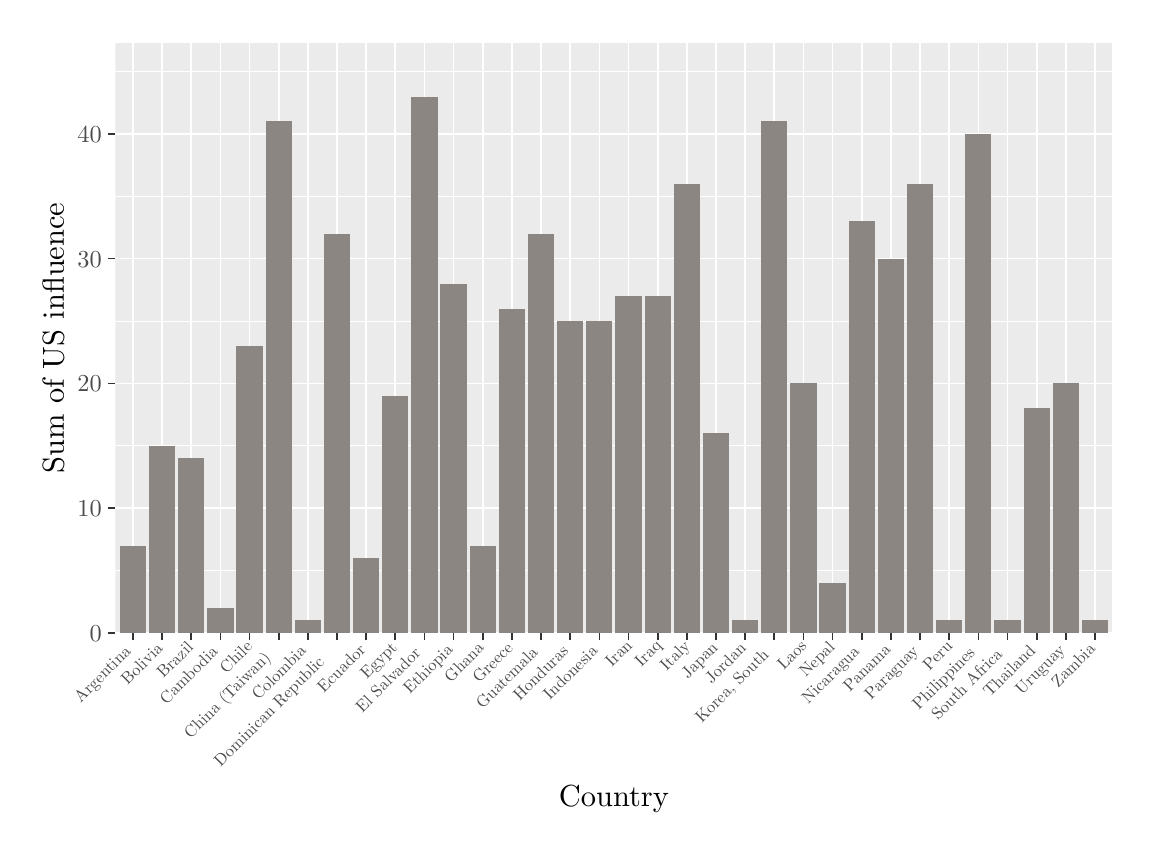
\begin{tikzpicture}[x=1pt,y=1pt]
\definecolor{fillColor}{RGB}{255,255,255}
\path[use as bounding box,fill=fillColor,fill opacity=0.00] (0,0) rectangle (397.48,289.08);
\begin{scope}
\path[clip] (  0.00,  0.00) rectangle (397.48,289.08);
\definecolor{drawColor}{RGB}{255,255,255}
\definecolor{fillColor}{RGB}{255,255,255}

\path[draw=drawColor,line width= 0.6pt,line join=round,line cap=round,fill=fillColor] (  0.00,  0.00) rectangle (397.48,289.08);
\end{scope}
\begin{scope}
\path[clip] ( 31.71, 70.39) rectangle (391.98,283.58);
\definecolor{fillColor}{gray}{0.92}

\path[fill=fillColor] ( 31.71, 70.39) rectangle (391.98,283.58);
\definecolor{drawColor}{RGB}{255,255,255}

\path[draw=drawColor,line width= 0.3pt,line join=round] ( 31.71, 92.93) --
	(391.98, 92.93);

\path[draw=drawColor,line width= 0.3pt,line join=round] ( 31.71,138.00) --
	(391.98,138.00);

\path[draw=drawColor,line width= 0.3pt,line join=round] ( 31.71,183.07) --
	(391.98,183.07);

\path[draw=drawColor,line width= 0.3pt,line join=round] ( 31.71,228.14) --
	(391.98,228.14);

\path[draw=drawColor,line width= 0.3pt,line join=round] ( 31.71,273.21) --
	(391.98,273.21);

\path[draw=drawColor,line width= 0.6pt,line join=round] ( 31.71, 70.39) --
	(391.98, 70.39);

\path[draw=drawColor,line width= 0.6pt,line join=round] ( 31.71,115.47) --
	(391.98,115.47);

\path[draw=drawColor,line width= 0.6pt,line join=round] ( 31.71,160.54) --
	(391.98,160.54);

\path[draw=drawColor,line width= 0.6pt,line join=round] ( 31.71,205.61) --
	(391.98,205.61);

\path[draw=drawColor,line width= 0.6pt,line join=round] ( 31.71,250.68) --
	(391.98,250.68);

\path[draw=drawColor,line width= 0.6pt,line join=round] ( 38.03, 70.39) --
	( 38.03,283.58);

\path[draw=drawColor,line width= 0.6pt,line join=round] ( 48.57, 70.39) --
	( 48.57,283.58);

\path[draw=drawColor,line width= 0.6pt,line join=round] ( 59.10, 70.39) --
	( 59.10,283.58);

\path[draw=drawColor,line width= 0.6pt,line join=round] ( 69.64, 70.39) --
	( 69.64,283.58);

\path[draw=drawColor,line width= 0.6pt,line join=round] ( 80.17, 70.39) --
	( 80.17,283.58);

\path[draw=drawColor,line width= 0.6pt,line join=round] ( 90.70, 70.39) --
	( 90.70,283.58);

\path[draw=drawColor,line width= 0.6pt,line join=round] (101.24, 70.39) --
	(101.24,283.58);

\path[draw=drawColor,line width= 0.6pt,line join=round] (111.77, 70.39) --
	(111.77,283.58);

\path[draw=drawColor,line width= 0.6pt,line join=round] (122.31, 70.39) --
	(122.31,283.58);

\path[draw=drawColor,line width= 0.6pt,line join=round] (132.84, 70.39) --
	(132.84,283.58);

\path[draw=drawColor,line width= 0.6pt,line join=round] (143.38, 70.39) --
	(143.38,283.58);

\path[draw=drawColor,line width= 0.6pt,line join=round] (153.91, 70.39) --
	(153.91,283.58);

\path[draw=drawColor,line width= 0.6pt,line join=round] (164.44, 70.39) --
	(164.44,283.58);

\path[draw=drawColor,line width= 0.6pt,line join=round] (174.98, 70.39) --
	(174.98,283.58);

\path[draw=drawColor,line width= 0.6pt,line join=round] (185.51, 70.39) --
	(185.51,283.58);

\path[draw=drawColor,line width= 0.6pt,line join=round] (196.05, 70.39) --
	(196.05,283.58);

\path[draw=drawColor,line width= 0.6pt,line join=round] (206.58, 70.39) --
	(206.58,283.58);

\path[draw=drawColor,line width= 0.6pt,line join=round] (217.12, 70.39) --
	(217.12,283.58);

\path[draw=drawColor,line width= 0.6pt,line join=round] (227.65, 70.39) --
	(227.65,283.58);

\path[draw=drawColor,line width= 0.6pt,line join=round] (238.18, 70.39) --
	(238.18,283.58);

\path[draw=drawColor,line width= 0.6pt,line join=round] (248.72, 70.39) --
	(248.72,283.58);

\path[draw=drawColor,line width= 0.6pt,line join=round] (259.25, 70.39) --
	(259.25,283.58);

\path[draw=drawColor,line width= 0.6pt,line join=round] (269.79, 70.39) --
	(269.79,283.58);

\path[draw=drawColor,line width= 0.6pt,line join=round] (280.32, 70.39) --
	(280.32,283.58);

\path[draw=drawColor,line width= 0.6pt,line join=round] (290.86, 70.39) --
	(290.86,283.58);

\path[draw=drawColor,line width= 0.6pt,line join=round] (301.39, 70.39) --
	(301.39,283.58);

\path[draw=drawColor,line width= 0.6pt,line join=round] (311.92, 70.39) --
	(311.92,283.58);

\path[draw=drawColor,line width= 0.6pt,line join=round] (322.46, 70.39) --
	(322.46,283.58);

\path[draw=drawColor,line width= 0.6pt,line join=round] (332.99, 70.39) --
	(332.99,283.58);

\path[draw=drawColor,line width= 0.6pt,line join=round] (343.53, 70.39) --
	(343.53,283.58);

\path[draw=drawColor,line width= 0.6pt,line join=round] (354.06, 70.39) --
	(354.06,283.58);

\path[draw=drawColor,line width= 0.6pt,line join=round] (364.60, 70.39) --
	(364.60,283.58);

\path[draw=drawColor,line width= 0.6pt,line join=round] (375.13, 70.39) --
	(375.13,283.58);

\path[draw=drawColor,line width= 0.6pt,line join=round] (385.66, 70.39) --
	(385.66,283.58);
\definecolor{fillColor}{RGB}{139,134,130}

\path[fill=fillColor] ( 33.29, 70.39) rectangle ( 42.77,101.94);

\path[fill=fillColor] ( 43.83, 70.39) rectangle ( 53.31,138.00);

\path[fill=fillColor] ( 54.36, 70.39) rectangle ( 63.84,133.49);

\path[fill=fillColor] ( 75.43, 70.39) rectangle ( 84.91,174.06);

\path[fill=fillColor] ( 96.50, 70.39) rectangle (105.98, 74.90);

\path[fill=fillColor] (107.03, 70.39) rectangle (116.51,214.62);

\path[fill=fillColor] (117.57, 70.39) rectangle (127.05, 97.44);

\path[fill=fillColor] (128.10, 70.39) rectangle (137.58,156.03);

\path[fill=fillColor] (149.17, 70.39) rectangle (158.65,196.59);

\path[fill=fillColor] (159.70, 70.39) rectangle (169.18,101.94);

\path[fill=fillColor] (170.24, 70.39) rectangle (179.72,187.58);

\path[fill=fillColor] (180.77, 70.39) rectangle (190.25,214.62);

\path[fill=fillColor] (191.31, 70.39) rectangle (200.79,183.07);

\path[fill=fillColor] (201.84, 70.39) rectangle (211.32,183.07);

\path[fill=fillColor] (212.38, 70.39) rectangle (221.86,192.09);

\path[fill=fillColor] (222.91, 70.39) rectangle (232.39,192.09);

\path[fill=fillColor] (233.44, 70.39) rectangle (242.92,232.65);

\path[fill=fillColor] (254.51, 70.39) rectangle (263.99, 74.90);

\path[fill=fillColor] (243.98, 70.39) rectangle (253.46,142.51);

\path[fill=fillColor] ( 64.90, 70.39) rectangle ( 74.38, 79.41);

\path[fill=fillColor] (265.05, 70.39) rectangle (274.53,255.19);

\path[fill=fillColor] (275.58, 70.39) rectangle (285.06,160.54);

\path[fill=fillColor] (296.65, 70.39) rectangle (306.13,219.13);

\path[fill=fillColor] (286.12, 70.39) rectangle (295.60, 88.42);

\path[fill=fillColor] (307.18, 70.39) rectangle (316.66,205.61);

\path[fill=fillColor] (328.25, 70.39) rectangle (337.73, 74.90);

\path[fill=fillColor] (338.79, 70.39) rectangle (348.27,250.68);

\path[fill=fillColor] (317.72, 70.39) rectangle (327.20,232.65);

\path[fill=fillColor] (138.64, 70.39) rectangle (148.12,264.20);

\path[fill=fillColor] (359.86, 70.39) rectangle (369.34,151.52);

\path[fill=fillColor] ( 85.96, 70.39) rectangle ( 95.44,255.19);

\path[fill=fillColor] (370.39, 70.39) rectangle (379.87,160.54);

\path[fill=fillColor] (349.32, 70.39) rectangle (358.80, 74.90);

\path[fill=fillColor] (380.92, 70.39) rectangle (390.40, 74.90);
\end{scope}
\begin{scope}
\path[clip] (  0.00,  0.00) rectangle (397.48,289.08);
\definecolor{drawColor}{gray}{0.30}

\node[text=drawColor,anchor=base east,inner sep=0pt, outer sep=0pt, scale=  0.88] at ( 26.76, 67.36) {0};

\node[text=drawColor,anchor=base east,inner sep=0pt, outer sep=0pt, scale=  0.88] at ( 26.76,112.44) {10};

\node[text=drawColor,anchor=base east,inner sep=0pt, outer sep=0pt, scale=  0.88] at ( 26.76,157.51) {20};

\node[text=drawColor,anchor=base east,inner sep=0pt, outer sep=0pt, scale=  0.88] at ( 26.76,202.58) {30};

\node[text=drawColor,anchor=base east,inner sep=0pt, outer sep=0pt, scale=  0.88] at ( 26.76,247.65) {40};
\end{scope}
\begin{scope}
\path[clip] (  0.00,  0.00) rectangle (397.48,289.08);
\definecolor{drawColor}{gray}{0.20}

\path[draw=drawColor,line width= 0.6pt,line join=round] ( 28.96, 70.39) --
	( 31.71, 70.39);

\path[draw=drawColor,line width= 0.6pt,line join=round] ( 28.96,115.47) --
	( 31.71,115.47);

\path[draw=drawColor,line width= 0.6pt,line join=round] ( 28.96,160.54) --
	( 31.71,160.54);

\path[draw=drawColor,line width= 0.6pt,line join=round] ( 28.96,205.61) --
	( 31.71,205.61);

\path[draw=drawColor,line width= 0.6pt,line join=round] ( 28.96,250.68) --
	( 31.71,250.68);
\end{scope}
\begin{scope}
\path[clip] (  0.00,  0.00) rectangle (397.48,289.08);
\definecolor{drawColor}{gray}{0.20}

\path[draw=drawColor,line width= 0.6pt,line join=round] ( 38.03, 67.64) --
	( 38.03, 70.39);

\path[draw=drawColor,line width= 0.6pt,line join=round] ( 48.57, 67.64) --
	( 48.57, 70.39);

\path[draw=drawColor,line width= 0.6pt,line join=round] ( 59.10, 67.64) --
	( 59.10, 70.39);

\path[draw=drawColor,line width= 0.6pt,line join=round] ( 69.64, 67.64) --
	( 69.64, 70.39);

\path[draw=drawColor,line width= 0.6pt,line join=round] ( 80.17, 67.64) --
	( 80.17, 70.39);

\path[draw=drawColor,line width= 0.6pt,line join=round] ( 90.70, 67.64) --
	( 90.70, 70.39);

\path[draw=drawColor,line width= 0.6pt,line join=round] (101.24, 67.64) --
	(101.24, 70.39);

\path[draw=drawColor,line width= 0.6pt,line join=round] (111.77, 67.64) --
	(111.77, 70.39);

\path[draw=drawColor,line width= 0.6pt,line join=round] (122.31, 67.64) --
	(122.31, 70.39);

\path[draw=drawColor,line width= 0.6pt,line join=round] (132.84, 67.64) --
	(132.84, 70.39);

\path[draw=drawColor,line width= 0.6pt,line join=round] (143.38, 67.64) --
	(143.38, 70.39);

\path[draw=drawColor,line width= 0.6pt,line join=round] (153.91, 67.64) --
	(153.91, 70.39);

\path[draw=drawColor,line width= 0.6pt,line join=round] (164.44, 67.64) --
	(164.44, 70.39);

\path[draw=drawColor,line width= 0.6pt,line join=round] (174.98, 67.64) --
	(174.98, 70.39);

\path[draw=drawColor,line width= 0.6pt,line join=round] (185.51, 67.64) --
	(185.51, 70.39);

\path[draw=drawColor,line width= 0.6pt,line join=round] (196.05, 67.64) --
	(196.05, 70.39);

\path[draw=drawColor,line width= 0.6pt,line join=round] (206.58, 67.64) --
	(206.58, 70.39);

\path[draw=drawColor,line width= 0.6pt,line join=round] (217.12, 67.64) --
	(217.12, 70.39);

\path[draw=drawColor,line width= 0.6pt,line join=round] (227.65, 67.64) --
	(227.65, 70.39);

\path[draw=drawColor,line width= 0.6pt,line join=round] (238.18, 67.64) --
	(238.18, 70.39);

\path[draw=drawColor,line width= 0.6pt,line join=round] (248.72, 67.64) --
	(248.72, 70.39);

\path[draw=drawColor,line width= 0.6pt,line join=round] (259.25, 67.64) --
	(259.25, 70.39);

\path[draw=drawColor,line width= 0.6pt,line join=round] (269.79, 67.64) --
	(269.79, 70.39);

\path[draw=drawColor,line width= 0.6pt,line join=round] (280.32, 67.64) --
	(280.32, 70.39);

\path[draw=drawColor,line width= 0.6pt,line join=round] (290.86, 67.64) --
	(290.86, 70.39);

\path[draw=drawColor,line width= 0.6pt,line join=round] (301.39, 67.64) --
	(301.39, 70.39);

\path[draw=drawColor,line width= 0.6pt,line join=round] (311.92, 67.64) --
	(311.92, 70.39);

\path[draw=drawColor,line width= 0.6pt,line join=round] (322.46, 67.64) --
	(322.46, 70.39);

\path[draw=drawColor,line width= 0.6pt,line join=round] (332.99, 67.64) --
	(332.99, 70.39);

\path[draw=drawColor,line width= 0.6pt,line join=round] (343.53, 67.64) --
	(343.53, 70.39);

\path[draw=drawColor,line width= 0.6pt,line join=round] (354.06, 67.64) --
	(354.06, 70.39);

\path[draw=drawColor,line width= 0.6pt,line join=round] (364.60, 67.64) --
	(364.60, 70.39);

\path[draw=drawColor,line width= 0.6pt,line join=round] (375.13, 67.64) --
	(375.13, 70.39);

\path[draw=drawColor,line width= 0.6pt,line join=round] (385.66, 67.64) --
	(385.66, 70.39);
\end{scope}
\begin{scope}
\path[clip] (  0.00,  0.00) rectangle (397.48,289.08);
\definecolor{drawColor}{gray}{0.30}

\node[text=drawColor,rotate= 45.00,anchor=base east,inner sep=0pt, outer sep=0pt, scale=  0.60] at ( 37.57, 63.30) {Argentina};

\node[text=drawColor,rotate= 45.00,anchor=base east,inner sep=0pt, outer sep=0pt, scale=  0.60] at ( 49.18, 64.37) {Bolivia};

\node[text=drawColor,rotate= 45.00,anchor=base east,inner sep=0pt, outer sep=0pt, scale=  0.60] at ( 60.11, 64.77) {Brazil};

\node[text=drawColor,rotate= 45.00,anchor=base east,inner sep=0pt, outer sep=0pt, scale=  0.60] at ( 69.06, 63.18) {Cambodia};

\node[text=drawColor,rotate= 45.00,anchor=base east,inner sep=0pt, outer sep=0pt, scale=  0.60] at ( 81.45, 65.05) {Chile};

\node[text=drawColor,rotate= 45.00,anchor=base east,inner sep=0pt, outer sep=0pt, scale=  0.60] at ( 88.07, 61.13) {China (Taiwan)};

\node[text=drawColor,rotate= 45.00,anchor=base east,inner sep=0pt, outer sep=0pt, scale=  0.60] at (100.94, 63.47) {Colombia};

\node[text=drawColor,rotate= 45.00,anchor=base east,inner sep=0pt, outer sep=0pt, scale=  0.60] at (107.45, 59.44) {Dominican Republic};

\node[text=drawColor,rotate= 45.00,anchor=base east,inner sep=0pt, outer sep=0pt, scale=  0.60] at (122.44, 63.90) {Ecuador};

\node[text=drawColor,rotate= 45.00,anchor=base east,inner sep=0pt, outer sep=0pt, scale=  0.60] at (133.81, 64.73) {Egypt};

\node[text=drawColor,rotate= 45.00,anchor=base east,inner sep=0pt, outer sep=0pt, scale=  0.60] at (142.31, 62.70) {El Salvador};

\node[text=drawColor,rotate= 45.00,anchor=base east,inner sep=0pt, outer sep=0pt, scale=  0.60] at (153.95, 63.81) {Ethiopia};

\node[text=drawColor,rotate= 45.00,anchor=base east,inner sep=0pt, outer sep=0pt, scale=  0.60] at (165.20, 64.52) {Ghana};

\node[text=drawColor,rotate= 45.00,anchor=base east,inner sep=0pt, outer sep=0pt, scale=  0.60] at (175.69, 64.47) {Greece};

\node[text=drawColor,rotate= 45.00,anchor=base east,inner sep=0pt, outer sep=0pt, scale=  0.60] at (184.67, 62.92) {Guatemala};

\node[text=drawColor,rotate= 45.00,anchor=base east,inner sep=0pt, outer sep=0pt, scale=  0.60] at (195.70, 63.41) {Honduras};

\node[text=drawColor,rotate= 45.00,anchor=base east,inner sep=0pt, outer sep=0pt, scale=  0.60] at (206.28, 63.46) {Indonesia};

\node[text=drawColor,rotate= 45.00,anchor=base east,inner sep=0pt, outer sep=0pt, scale=  0.60] at (218.80, 65.44) {Iran};

\node[text=drawColor,rotate= 45.00,anchor=base east,inner sep=0pt, outer sep=0pt, scale=  0.60] at (229.35, 65.47) {Iraq};

\node[text=drawColor,rotate= 45.00,anchor=base east,inner sep=0pt, outer sep=0pt, scale=  0.60] at (239.65, 65.23) {Italy};

\node[text=drawColor,rotate= 45.00,anchor=base east,inner sep=0pt, outer sep=0pt, scale=  0.60] at (249.71, 64.75) {Japan};

\node[text=drawColor,rotate= 45.00,anchor=base east,inner sep=0pt, outer sep=0pt, scale=  0.60] at (259.91, 64.42) {Jordan};

\node[text=drawColor,rotate= 45.00,anchor=base east,inner sep=0pt, outer sep=0pt, scale=  0.60] at (268.12, 62.10) {Korea, South};

\node[text=drawColor,rotate= 45.00,anchor=base east,inner sep=0pt, outer sep=0pt, scale=  0.60] at (281.82, 65.27) {Laos};

\node[text=drawColor,rotate= 45.00,anchor=base east,inner sep=0pt, outer sep=0pt, scale=  0.60] at (291.93, 64.83) {Nepal};

\node[text=drawColor,rotate= 45.00,anchor=base east,inner sep=0pt, outer sep=0pt, scale=  0.60] at (300.86, 63.23) {Nicaragua};

\node[text=drawColor,rotate= 45.00,anchor=base east,inner sep=0pt, outer sep=0pt, scale=  0.60] at (312.13, 63.97) {Panama};

\node[text=drawColor,rotate= 45.00,anchor=base east,inner sep=0pt, outer sep=0pt, scale=  0.60] at (322.19, 63.50) {Paraguay};

\node[text=drawColor,rotate= 45.00,anchor=base east,inner sep=0pt, outer sep=0pt, scale=  0.60] at (334.47, 65.24) {Peru};

\node[text=drawColor,rotate= 45.00,anchor=base east,inner sep=0pt, outer sep=0pt, scale=  0.60] at (342.62, 62.86) {Philippines};

\node[text=drawColor,rotate= 45.00,anchor=base east,inner sep=0pt, outer sep=0pt, scale=  0.60] at (352.56, 62.26) {South Africa};

\node[text=drawColor,rotate= 45.00,anchor=base east,inner sep=0pt, outer sep=0pt, scale=  0.60] at (364.46, 63.63) {Thailand};

\node[text=drawColor,rotate= 45.00,anchor=base east,inner sep=0pt, outer sep=0pt, scale=  0.60] at (375.16, 63.80) {Uruguay};

\node[text=drawColor,rotate= 45.00,anchor=base east,inner sep=0pt, outer sep=0pt, scale=  0.60] at (386.12, 64.22) {Zambia};
\end{scope}
\begin{scope}
\path[clip] (  0.00,  0.00) rectangle (397.48,289.08);
\definecolor{drawColor}{RGB}{0,0,0}

\node[text=drawColor,anchor=base,inner sep=0pt, outer sep=0pt, scale=  1.10] at (211.85,  7.64) {Country};
\end{scope}
\begin{scope}
\path[clip] (  0.00,  0.00) rectangle (397.48,289.08);
\definecolor{drawColor}{RGB}{0,0,0}

\node[text=drawColor,rotate= 90.00,anchor=base,inner sep=0pt, outer sep=0pt, scale=  1.10] at ( 13.08,176.99) {Sum of US influence};
\end{scope}
\end{tikzpicture}

\caption{US influence by country}
\end{figure}

\begin{figure}[ht]
% Created by tikzDevice version 0.12.3.1 on 2021-04-04 17:56:42
% !TEX encoding = UTF-8 Unicode
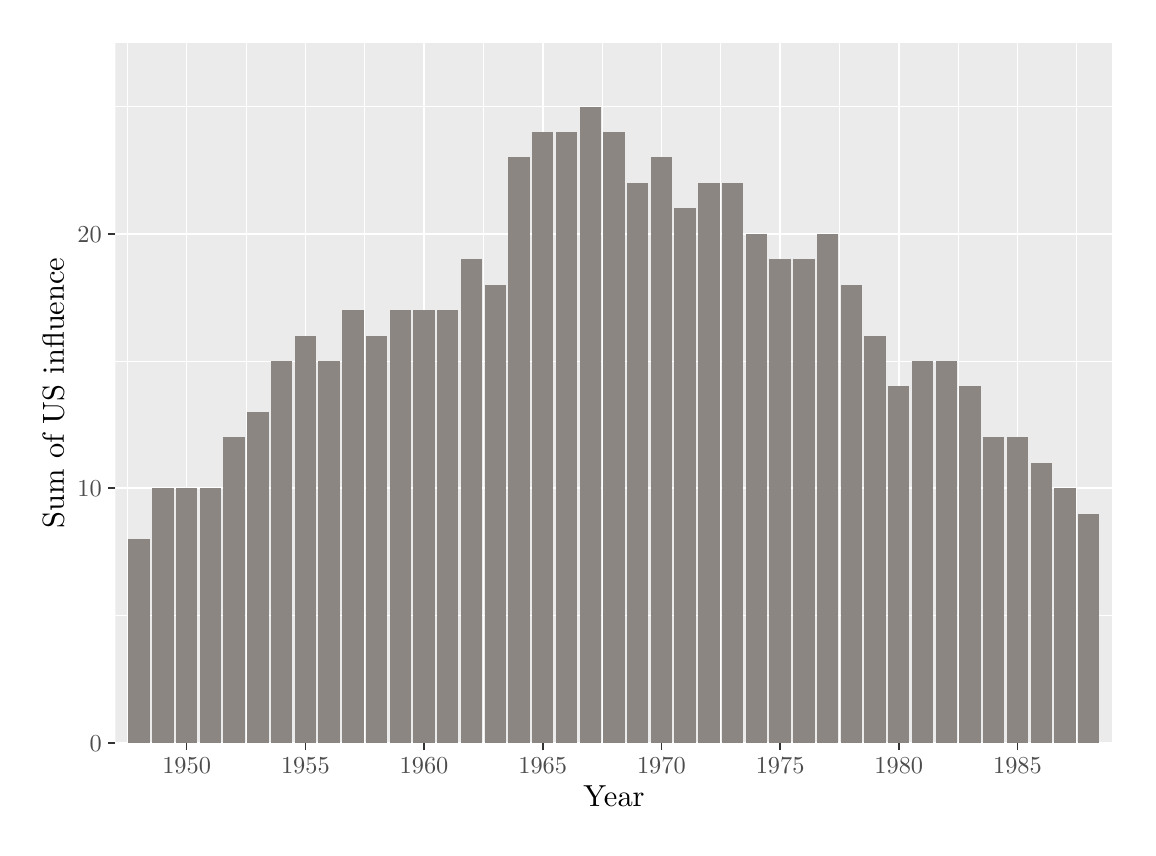
\begin{tikzpicture}[x=1pt,y=1pt]
\definecolor{fillColor}{RGB}{255,255,255}
\path[use as bounding box,fill=fillColor,fill opacity=0.00] (0,0) rectangle (397.48,289.08);
\begin{scope}
\path[clip] (  0.00,  0.00) rectangle (397.48,289.08);
\definecolor{drawColor}{RGB}{255,255,255}
\definecolor{fillColor}{RGB}{255,255,255}

\path[draw=drawColor,line width= 0.6pt,line join=round,line cap=round,fill=fillColor] (  0.00,  0.00) rectangle (397.48,289.08);
\end{scope}
\begin{scope}
\path[clip] ( 31.71, 30.69) rectangle (391.98,283.58);
\definecolor{fillColor}{gray}{0.92}

\path[fill=fillColor] ( 31.71, 30.69) rectangle (391.98,283.58);
\definecolor{drawColor}{RGB}{255,255,255}

\path[draw=drawColor,line width= 0.3pt,line join=round] ( 31.71, 76.67) --
	(391.98, 76.67);

\path[draw=drawColor,line width= 0.3pt,line join=round] ( 31.71,168.63) --
	(391.98,168.63);

\path[draw=drawColor,line width= 0.3pt,line join=round] ( 31.71,260.59) --
	(391.98,260.59);

\path[draw=drawColor,line width= 0.3pt,line join=round] ( 36.00, 30.69) --
	( 36.00,283.58);

\path[draw=drawColor,line width= 0.3pt,line join=round] ( 78.89, 30.69) --
	( 78.89,283.58);

\path[draw=drawColor,line width= 0.3pt,line join=round] (121.78, 30.69) --
	(121.78,283.58);

\path[draw=drawColor,line width= 0.3pt,line join=round] (164.67, 30.69) --
	(164.67,283.58);

\path[draw=drawColor,line width= 0.3pt,line join=round] (207.56, 30.69) --
	(207.56,283.58);

\path[draw=drawColor,line width= 0.3pt,line join=round] (250.45, 30.69) --
	(250.45,283.58);

\path[draw=drawColor,line width= 0.3pt,line join=round] (293.34, 30.69) --
	(293.34,283.58);

\path[draw=drawColor,line width= 0.3pt,line join=round] (336.23, 30.69) --
	(336.23,283.58);

\path[draw=drawColor,line width= 0.3pt,line join=round] (379.12, 30.69) --
	(379.12,283.58);

\path[draw=drawColor,line width= 0.6pt,line join=round] ( 31.71, 30.69) --
	(391.98, 30.69);

\path[draw=drawColor,line width= 0.6pt,line join=round] ( 31.71,122.65) --
	(391.98,122.65);

\path[draw=drawColor,line width= 0.6pt,line join=round] ( 31.71,214.61) --
	(391.98,214.61);

\path[draw=drawColor,line width= 0.6pt,line join=round] ( 57.45, 30.69) --
	( 57.45,283.58);

\path[draw=drawColor,line width= 0.6pt,line join=round] (100.34, 30.69) --
	(100.34,283.58);

\path[draw=drawColor,line width= 0.6pt,line join=round] (143.23, 30.69) --
	(143.23,283.58);

\path[draw=drawColor,line width= 0.6pt,line join=round] (186.11, 30.69) --
	(186.11,283.58);

\path[draw=drawColor,line width= 0.6pt,line join=round] (229.00, 30.69) --
	(229.00,283.58);

\path[draw=drawColor,line width= 0.6pt,line join=round] (271.89, 30.69) --
	(271.89,283.58);

\path[draw=drawColor,line width= 0.6pt,line join=round] (314.78, 30.69) --
	(314.78,283.58);

\path[draw=drawColor,line width= 0.6pt,line join=round] (357.67, 30.69) --
	(357.67,283.58);
\definecolor{fillColor}{RGB}{139,134,130}

\path[fill=fillColor] ( 36.43, 30.69) rectangle ( 44.15,104.26);

\path[fill=fillColor] ( 45.01, 30.69) rectangle ( 52.73,122.65);

\path[fill=fillColor] ( 53.59, 30.69) rectangle ( 61.31,122.65);

\path[fill=fillColor] ( 62.16, 30.69) rectangle ( 69.88,122.65);

\path[fill=fillColor] ( 70.74, 30.69) rectangle ( 78.46,141.04);

\path[fill=fillColor] ( 79.32, 30.69) rectangle ( 87.04,150.24);

\path[fill=fillColor] ( 87.90, 30.69) rectangle ( 95.62,168.63);

\path[fill=fillColor] ( 96.48, 30.69) rectangle (104.20,177.82);

\path[fill=fillColor] (105.05, 30.69) rectangle (112.77,168.63);

\path[fill=fillColor] (113.63, 30.69) rectangle (121.35,187.02);

\path[fill=fillColor] (122.21, 30.69) rectangle (129.93,177.82);

\path[fill=fillColor] (130.79, 30.69) rectangle (138.51,187.02);

\path[fill=fillColor] (139.37, 30.69) rectangle (147.09,187.02);

\path[fill=fillColor] (147.94, 30.69) rectangle (155.66,187.02);

\path[fill=fillColor] (156.52, 30.69) rectangle (164.24,205.41);

\path[fill=fillColor] (165.10, 30.69) rectangle (172.82,196.22);

\path[fill=fillColor] (173.68, 30.69) rectangle (181.40,242.20);

\path[fill=fillColor] (182.25, 30.69) rectangle (189.97,251.39);

\path[fill=fillColor] (190.83, 30.69) rectangle (198.55,251.39);

\path[fill=fillColor] (199.41, 30.69) rectangle (207.13,260.59);

\path[fill=fillColor] (207.99, 30.69) rectangle (215.71,251.39);

\path[fill=fillColor] (216.57, 30.69) rectangle (224.29,233.00);

\path[fill=fillColor] (225.14, 30.69) rectangle (232.86,242.20);

\path[fill=fillColor] (233.72, 30.69) rectangle (241.44,223.81);

\path[fill=fillColor] (242.30, 30.69) rectangle (250.02,233.00);

\path[fill=fillColor] (250.88, 30.69) rectangle (258.60,233.00);

\path[fill=fillColor] (259.46, 30.69) rectangle (267.18,214.61);

\path[fill=fillColor] (268.03, 30.69) rectangle (275.75,205.41);

\path[fill=fillColor] (276.61, 30.69) rectangle (284.33,205.41);

\path[fill=fillColor] (285.19, 30.69) rectangle (292.91,214.61);

\path[fill=fillColor] (293.77, 30.69) rectangle (301.49,196.22);

\path[fill=fillColor] (302.35, 30.69) rectangle (310.07,177.82);

\path[fill=fillColor] (310.92, 30.69) rectangle (318.64,159.43);

\path[fill=fillColor] (319.50, 30.69) rectangle (327.22,168.63);

\path[fill=fillColor] (328.08, 30.69) rectangle (335.80,168.63);

\path[fill=fillColor] (336.66, 30.69) rectangle (344.38,159.43);

\path[fill=fillColor] (345.24, 30.69) rectangle (352.96,141.04);

\path[fill=fillColor] (353.81, 30.69) rectangle (361.53,141.04);

\path[fill=fillColor] (362.39, 30.69) rectangle (370.11,131.84);

\path[fill=fillColor] (370.97, 30.69) rectangle (378.69,122.65);

\path[fill=fillColor] (379.55, 30.69) rectangle (387.27,113.45);
\end{scope}
\begin{scope}
\path[clip] (  0.00,  0.00) rectangle (397.48,289.08);
\definecolor{drawColor}{gray}{0.30}

\node[text=drawColor,anchor=base east,inner sep=0pt, outer sep=0pt, scale=  0.88] at ( 26.76, 27.66) {0};

\node[text=drawColor,anchor=base east,inner sep=0pt, outer sep=0pt, scale=  0.88] at ( 26.76,119.62) {10};

\node[text=drawColor,anchor=base east,inner sep=0pt, outer sep=0pt, scale=  0.88] at ( 26.76,211.58) {20};
\end{scope}
\begin{scope}
\path[clip] (  0.00,  0.00) rectangle (397.48,289.08);
\definecolor{drawColor}{gray}{0.20}

\path[draw=drawColor,line width= 0.6pt,line join=round] ( 28.96, 30.69) --
	( 31.71, 30.69);

\path[draw=drawColor,line width= 0.6pt,line join=round] ( 28.96,122.65) --
	( 31.71,122.65);

\path[draw=drawColor,line width= 0.6pt,line join=round] ( 28.96,214.61) --
	( 31.71,214.61);
\end{scope}
\begin{scope}
\path[clip] (  0.00,  0.00) rectangle (397.48,289.08);
\definecolor{drawColor}{gray}{0.20}

\path[draw=drawColor,line width= 0.6pt,line join=round] ( 57.45, 27.94) --
	( 57.45, 30.69);

\path[draw=drawColor,line width= 0.6pt,line join=round] (100.34, 27.94) --
	(100.34, 30.69);

\path[draw=drawColor,line width= 0.6pt,line join=round] (143.23, 27.94) --
	(143.23, 30.69);

\path[draw=drawColor,line width= 0.6pt,line join=round] (186.11, 27.94) --
	(186.11, 30.69);

\path[draw=drawColor,line width= 0.6pt,line join=round] (229.00, 27.94) --
	(229.00, 30.69);

\path[draw=drawColor,line width= 0.6pt,line join=round] (271.89, 27.94) --
	(271.89, 30.69);

\path[draw=drawColor,line width= 0.6pt,line join=round] (314.78, 27.94) --
	(314.78, 30.69);

\path[draw=drawColor,line width= 0.6pt,line join=round] (357.67, 27.94) --
	(357.67, 30.69);
\end{scope}
\begin{scope}
\path[clip] (  0.00,  0.00) rectangle (397.48,289.08);
\definecolor{drawColor}{gray}{0.30}

\node[text=drawColor,anchor=base,inner sep=0pt, outer sep=0pt, scale=  0.88] at ( 57.45, 19.68) {1950};

\node[text=drawColor,anchor=base,inner sep=0pt, outer sep=0pt, scale=  0.88] at (100.34, 19.68) {1955};

\node[text=drawColor,anchor=base,inner sep=0pt, outer sep=0pt, scale=  0.88] at (143.23, 19.68) {1960};

\node[text=drawColor,anchor=base,inner sep=0pt, outer sep=0pt, scale=  0.88] at (186.11, 19.68) {1965};

\node[text=drawColor,anchor=base,inner sep=0pt, outer sep=0pt, scale=  0.88] at (229.00, 19.68) {1970};

\node[text=drawColor,anchor=base,inner sep=0pt, outer sep=0pt, scale=  0.88] at (271.89, 19.68) {1975};

\node[text=drawColor,anchor=base,inner sep=0pt, outer sep=0pt, scale=  0.88] at (314.78, 19.68) {1980};

\node[text=drawColor,anchor=base,inner sep=0pt, outer sep=0pt, scale=  0.88] at (357.67, 19.68) {1985};
\end{scope}
\begin{scope}
\path[clip] (  0.00,  0.00) rectangle (397.48,289.08);
\definecolor{drawColor}{RGB}{0,0,0}

\node[text=drawColor,anchor=base,inner sep=0pt, outer sep=0pt, scale=  1.10] at (211.85,  7.64) {Year};
\end{scope}
\begin{scope}
\path[clip] (  0.00,  0.00) rectangle (397.48,289.08);
\definecolor{drawColor}{RGB}{0,0,0}

\node[text=drawColor,rotate= 90.00,anchor=base,inner sep=0pt, outer sep=0pt, scale=  1.10] at ( 13.08,157.13) {Sum of US influence};
\end{scope}
\end{tikzpicture}

\caption{US influence by year}
\end{figure}


\par{As noted in the \citet{berger2013superpower}, the variable encoded is specifically for covert CIA interventions, hence its motivation is not subject to public opinion. This nicely removes at least one source of endogeneity in my estimating equations. Another important aspect of this variable is that, as \citet{berger2013superpower} argue, it measures ``client states" or ``puppet leaders"---in particular, whether or not the US has close ties with the foreign government in a particular country and year. This aspect of the variable provides the crux of my mechanism, through which the US could influence both the political elite and the policies of foreign governments---in particular, those that work in favor of US, the foreign government, and US and foreign business economic interests while coming at the expense of other priorities such as public provisions.}
\par{The data from which the controls for democracy, economic left-right policy, welfare policy, and union membership are from the Varieties of Democracy (V-Dem) \citep{vdem} Project, version 11, with the latter two measures coming from the Varieties of Party Identity and Organisation (V-Party) \citep{vparty} dataset. The inclusion of democracy as a control is natural as it is expected to affect both the US decision to intervene \citep{mullenbach2008deciding} and income inequality via the mechanism proposed by \citet{bueno2006intervention} whereby more democratic governments require larger winning coalitions to stay in power and as a result must provide more public goods to retain a large coalition. In the V-Dem dataset, several measures of democracy are presented, including electoral, liberal, participatory, and deliberative, however, as noted in the V-Dem Codebook \citep{coppedge2021v}, electoral democracy is an essential aspect of all the other measures, as it captures the extent to which elections are clean, fair, and open to the entire population. Hence, I have chosen to use electoral democracy.}
\par{As for the economic left-right control variable, which as described in the V-Party Codebook \citep{luhrmann2020v} essentially captures the extent to which a political party favors increased government spending, regulation, and taxes as opposed to less spending, privatization, and lower taxes. It is coded as a sliding scale centered at zero where more negative values means more left and more positive means more right. The welfare variable more specifically captures whether or not the party supports universal welfare or means-tested welfare, where more negative values means more means-tested or no welfare policy and more positive values means more universal welfare policies. As both of these variables are by political party and not by country, I weigh the variables for each party by the share of seats that party held in government, then summed the variables for each country-year pair to get the average of the government's position on these policies. The limitations of this methodology include that the system of government may lend itself to majority rule, in which case weighing the minority parties by seat share may overestimate their real influence on government policy. Further research may expand upon this limitation, but for the purposes of my study, I find these metrics a useful control when considering income inequality. Finally, the share of the population involved in independent trade unions variable is measured such that more positive values indicate a larger share of the population involved, and this variable is relevant in its relationship to wages via collective bargaining on the part of the union, which in turn is likely to affect measures of income inequality.}
\par{The data for per capita GDP comes from the Maddison Project Database, version 2020 \citep{maddison}, and I use log GDP per capita as per \citet{berger2013superpower}. Table 1 below shows the summary statistics for each of the dependent, explanatory, and control variables.}

\begin{table}[ht]
\caption{Summary statistics}
\centering
\begin{tabular}{lrrrrr}
\toprule
 Variables & Obs & Mean & StdDev & Min & Max \\ 
  \midrule
 Median Gini & 3092 & 37.61 & 9.26 & 15.90 & 73.25 \\ 
   Median Top 10 Share & 2492 & 29.50 & 7.36 & 16.39 & 64.79 \\ 
   US intervention & 3882 & 0.18 & 0.38 & 0.00 & 1.00 \\ 
   Democracy & 2956 & 0.62 & 0.26 & 0.05 & 0.92 \\ 
   Economic Left-Right & 755 & 0.15 & 0.66 & -3.54 & 2.68 \\ 
   Welfare Policy & 755 & 0.10 & 0.84 & -2.73 & 3.08 \\ 
   Union Membership & 2918 & 0.58 & 1.24 & -3.12 & 3.61 \\ 
   GDP Per Capita & 2963 & 9.32 & 1.00 & 6.55 & 11.35 \\ 
   \bottomrule
\end{tabular}

\end{table}



% FIGURE 1: US INTVNS BY YEAR
% FIGURE 2: US INTVNS BY COUNTRY

%%%%%%%%%%%%%%%% EQUATIONS & METHODS %%%%%%%%%%%%%%%%%%%%
\section{Estimating equations and methods}
\par{As I am interested in the within-country relationship between US influence and income inequality, I estimate the following equation}
\begin{equation}
	Y_{c,t} = \alpha y_{c,t-1} + \beta I_{c,t} + \gamma X{c,t} + \mu_c + \mu_t + \varepsilon_{c,t}
\end{equation}
with $c$ indexing the variables by country and $t$ indexing by year for the period 1947-2019. $Y_{c,t}$ captures the dependent variables of interest, which are the measures of inequality that include the Gini coefficient and top ten percent share of income or consumption. The explanatory variables include a lagged dependent variable, $y_{c,t-1}$, which is included to control for persistence in income inequality. If the coefficient on this variable is positive, it means the magnitude of the effects of the other explanatory variables, in particular US influence, is greater. If this coefficient is negative, it would imply a tendency of inequality to revert to its mean between years, implying a diminished effect of US influence. However, the use of a lagged dependent variable, known as a dynamic panel model, introduces a potential source of bias, called Nickell bias, where the lagged dependent variable is correlated with the error term via the fixed-effects demeaning process. Following \citet{berger2013superpower}, I claim my sample is not subject to Nickell bias due to a sufficiently large $T$, or time frame.
\par{The explanatory variables are US influence, or $I_{c,t}$, the control variables grouped in $X_{c,t}$, and the country and year fixed effects variables, $\mu_c$ and $\mu_t$, which control for omitted variables for each given country and year.}





%%%%%%%%%%%%%%%% RESULTS & DISCUSSION %%%%%%%%%%%%%%%%%%%%
\section{Results}

\par{The results for the effect of US influence on the Gini coefficient are shown in Table 2 below. The estimating equation is as described above, with country and year fixed effects included in all regressions in addition to the Gini coefficient lagged by one year, electoral democracy, union membership, and log GDP per capita as controls. Other controls, namely economic left-right scale and welfare policy, have not been included in Table 2 due to their  small number of observations which signficantly reduced the $N$ for the regressions. The explanatory variable of interest, $I_{t,c}$, is lagged an additional year in each consecutive regression, from a one-year lag to a 30-year lag. This accounts for the expected delay in effects on measures of inequality, as each regression shows the average effect of US influence on inequality $t$-years after a CIA intervention to install or support a regime.}
\par{The results for the effect on the Gini coefficient support my hypothesis, as every coefficient for lagged US influence is positive and statistically significant for each of the first 25 years, after which it remains positive but insignficiant. The interpretation of this coefficient ($\beta$) is that if a country experienced a covert CIA intervention in a particular year, then the Gini coefficient is expected to rise by $\beta$ in that country $t$ years later where $t$ is equal to the year lag on US influence. Contrary to \citet{berger2013superpower}, which studied the effects of US influence on long-run democracy and found significant effects within a decade of the end of an intervention but a decay in effects to insignificance in the long-run, my results suggest a significant and persistent effect of US influence on inequality.}


\begin{table}
\caption{US influence on Gini coefficient}
\begin{center}
\begin{tabular}{l c c c c c c}
\toprule
 & 1-Year Lag & 2-Year & 3-Year & 4-Year & 5-Year & 6-Year \\
\midrule
US influence        & $\mathbf{2.05}^{***}$ & $\mathbf{1.90}^{***}$ & $\mathbf{1.69}^{***}$ & $\mathbf{1.59}^{**}$  & $\mathbf{1.20}^{*}$   & $\mathbf{1.44}^{**}$  \\
                    & $(0.57)$              & $(0.52)$              & $(0.50)$              & $(0.49)$              & $(0.47)$              & $(0.44)$              \\
Gini (t-1)          & $\mathbf{0.62}^{***}$ & $\mathbf{0.65}^{***}$ & $\mathbf{0.65}^{***}$ & $\mathbf{0.62}^{***}$ & $\mathbf{0.62}^{***}$ & $\mathbf{0.62}^{***}$ \\
                    & $(0.02)$              & $(0.02)$              & $(0.02)$              & $(0.02)$              & $(0.02)$              & $(0.02)$              \\
Electoral Democracy & $0.62$                & $0.21$                & $0.21$                & $-0.19$               & $-0.58$               & $-0.14$               \\
                    & $(0.90)$              & $(0.87)$              & $(0.85)$              & $(0.87)$              & $(0.86)$              & $(0.84)$              \\
Union Membership    & $0.20$                & $0.22$                & $0.15$                & $0.29$                & $0.32$                & $0.26$                \\
                    & $(0.21)$              & $(0.20)$              & $(0.20)$              & $(0.21)$              & $(0.21)$              & $(0.20)$              \\
Log GDP Per Capita  & $-0.35$               & $-0.31$               & $-0.24$               & $-0.51$               & $-0.58$               & $-0.48$               \\
                    & $(0.49)$              & $(0.47)$              & $(0.47)$              & $(0.48)$              & $(0.48)$              & $(0.48)$              \\
\midrule
R$^2$               & $0.44$                & $0.46$                & $0.46$                & $0.44$                & $0.44$                & $0.44$                \\
Adj. R$^2$          & $0.37$                & $0.40$                & $0.40$                & $0.37$                & $0.38$                & $0.38$                \\
Num. obs.           & $1461$                & $1459$                & $1454$                & $1460$                & $1448$                & $1441$                \\
\bottomrule
\multicolumn{7}{l}{\scriptsize{$^{***}p<0.001$; $^{**}p<0.01$; $^{*}p<0.05$}}
\end{tabular}
\label{table:coefficients}
\end{center}
\end{table}


\begin{table}
\begin{center}
\begin{tabular}{l c c c c c c}
\toprule
 & 7-Year Lag & 8-Year & 9-Year & 10-Year & 11-Year & 12-Year \\
\midrule
US influence        & $\mathbf{1.93}^{***}$ & $\mathbf{1.79}^{***}$ & $\mathbf{1.90}^{***}$ & $\mathbf{1.95}^{***}$ & $\mathbf{1.86}^{***}$ & $\mathbf{1.89}^{***}$ \\
                    & $(0.41)$              & $(0.39)$              & $(0.38)$              & $(0.36)$              & $(0.35)$              & $(0.34)$              \\
Gini (t-1)          & $\mathbf{0.60}^{***}$ & $\mathbf{0.60}^{***}$ & $\mathbf{0.60}^{***}$ & $\mathbf{0.60}^{***}$ & $\mathbf{0.60}^{***}$ & $\mathbf{0.60}^{***}$ \\
                    & $(0.02)$              & $(0.02)$              & $(0.02)$              & $(0.02)$              & $(0.02)$              & $(0.02)$              \\
Electoral Democracy & $-0.34$               & $-0.22$               & $-0.53$               & $-0.40$               & $-0.52$               & $-0.57$               \\
                    & $(0.83)$              & $(0.82)$              & $(0.83)$              & $(0.82)$              & $(0.81)$              & $(0.81)$              \\
Union Membership    & $0.38$                & $0.39$                & $\mathbf{0.46}^{*}$   & $\mathbf{0.47}^{*}$   & $\mathbf{0.44}^{*}$   & $\mathbf{0.48}^{*}$   \\
                    & $(0.20)$              & $(0.20)$              & $(0.20)$              & $(0.20)$              & $(0.20)$              & $(0.20)$              \\
Log GDP Per Capita  & $-0.47$               & $-0.54$               & $-0.47$               & $-0.57$               & $-0.41$               & $-0.43$               \\
                    & $(0.47)$              & $(0.48)$              & $(0.47)$              & $(0.47)$              & $(0.47)$              & $(0.47)$              \\
\midrule
R$^2$               & $0.44$                & $0.43$                & $0.43$                & $0.43$                & $0.44$                & $0.44$                \\
Adj. R$^2$          & $0.38$                & $0.37$                & $0.37$                & $0.37$                & $0.38$                & $0.38$                \\
Num. obs.           & $1441$                & $1439$                & $1438$                & $1439$                & $1433$                & $1431$                \\
\bottomrule
\multicolumn{7}{l}{\scriptsize{$^{***}p<0.001$; $^{**}p<0.01$; $^{*}p<0.05$}}
\end{tabular}
\label{table:coefficients}
\end{center}
\end{table}


\begin{table}
\begin{center}
\begin{tabular}{l c c c c c c}
\toprule
 & 13-Year Lag & 14-Year & 15-Year & 16-Year & 17-Year & 18-Year \\
\midrule
US influence        & $\mathbf{1.82}^{***}$ & $\mathbf{1.47}^{***}$ & $\mathbf{1.55}^{***}$ & $\mathbf{1.56}^{***}$ & $\mathbf{1.54}^{***}$ & $\mathbf{1.56}^{***}$ \\
                    & $(0.33)$              & $(0.33)$              & $(0.32)$              & $(0.32)$              & $(0.31)$              & $(0.31)$              \\
Gini (t-1)          & $\mathbf{0.61}^{***}$ & $\mathbf{0.62}^{***}$ & $\mathbf{0.62}^{***}$ & $\mathbf{0.61}^{***}$ & $\mathbf{0.62}^{***}$ & $\mathbf{0.62}^{***}$ \\
                    & $(0.02)$              & $(0.02)$              & $(0.02)$              & $(0.02)$              & $(0.02)$              & $(0.02)$              \\
Electoral Democracy & $-0.61$               & $-0.74$               & $-0.94$               & $-0.99$               & $-1.13$               & $-1.05$               \\
                    & $(0.81)$              & $(0.81)$              & $(0.80)$              & $(0.81)$              & $(0.81)$              & $(0.81)$              \\
Union Membership    & $\mathbf{0.47}^{*}$   & $\mathbf{0.44}^{*}$   & $\mathbf{0.50}^{*}$   & $\mathbf{0.49}^{*}$   & $\mathbf{0.51}^{*}$   & $\mathbf{0.49}^{*}$   \\
                    & $(0.20)$              & $(0.20)$              & $(0.20)$              & $(0.20)$              & $(0.20)$              & $(0.20)$              \\
Log GDP Per Capita  & $-0.62$               & $-0.59$               & $-0.61$               & $-0.63$               & $-0.66$               & $-0.70$               \\
                    & $(0.47)$              & $(0.47)$              & $(0.47)$              & $(0.47)$              & $(0.49)$              & $(0.49)$              \\
\midrule
R$^2$               & $0.44$                & $0.44$                & $0.44$                & $0.44$                & $0.44$                & $0.44$                \\
Adj. R$^2$          & $0.39$                & $0.39$                & $0.39$                & $0.38$                & $0.38$                & $0.38$                \\
Num. obs.           & $1430$                & $1426$                & $1421$                & $1417$                & $1413$                & $1404$                \\
\bottomrule
\multicolumn{7}{l}{\scriptsize{$^{***}p<0.001$; $^{**}p<0.01$; $^{*}p<0.05$}}
\end{tabular}
\label{table:coefficients}
\end{center}
\end{table}


\begin{table}
\begin{center}
\begin{tabular}{l c c c c c c}
\toprule
 & 19-Year Lag & 20-Year & 21-Year & 22-Year & 23-Year & 24-Year \\
\midrule
US infuence         & $\mathbf{1.48}^{***}$ & $\mathbf{1.19}^{***}$ & $\mathbf{0.98}^{**}$  & $\mathbf{1.02}^{***}$ & $\mathbf{0.81}^{**}$  & $\mathbf{0.74}^{*}$   \\
                    & $(0.31)$              & $(0.31)$              & $(0.30)$              & $(0.30)$              & $(0.30)$              & $(0.32)$              \\
Gini (t-1)          & $\mathbf{0.62}^{***}$ & $\mathbf{0.62}^{***}$ & $\mathbf{0.63}^{***}$ & $\mathbf{0.66}^{***}$ & $\mathbf{0.66}^{***}$ & $\mathbf{0.62}^{***}$ \\
                    & $(0.02)$              & $(0.02)$              & $(0.02)$              & $(0.02)$              & $(0.02)$              & $(0.02)$              \\
Electoral Democracy & $-1.03$               & $-1.35$               & $-1.01$               & $\mathbf{-1.55}^{*}$  & $-1.42$               & $-1.03$               \\
                    & $(0.81)$              & $(0.81)$              & $(0.80)$              & $(0.77)$              & $(0.78)$              & $(0.84)$              \\
Union Membership    & $\mathbf{0.50}^{*}$   & $\mathbf{0.47}^{*}$   & $\mathbf{0.41}^{*}$   & $\mathbf{0.48}^{*}$   & $0.39$                & $0.38$                \\
                    & $(0.20)$              & $(0.20)$              & $(0.20)$              & $(0.19)$              & $(0.20)$              & $(0.21)$              \\
Log GDP Per Capita  & $-0.53$               & $-0.63$               & $-0.68$               & $-0.42$               & $-0.35$               & $-0.45$               \\
                    & $(0.49)$              & $(0.49)$              & $(0.49)$              & $(0.47)$              & $(0.48)$              & $(0.51)$              \\
\midrule
R$^2$               & $0.44$                & $0.44$                & $0.44$                & $0.47$                & $0.46$                & $0.42$                \\
Adj. R$^2$          & $0.38$                & $0.38$                & $0.39$                & $0.42$                & $0.41$                & $0.36$                \\
Num. obs.           & $1399$                & $1399$                & $1392$                & $1382$                & $1379$                & $1369$                \\
\bottomrule
\multicolumn{7}{l}{\scriptsize{$^{***}p<0.001$; $^{**}p<0.01$; $^{*}p<0.05$}}
\end{tabular}
\label{table:coefficients}
\end{center}
\end{table}


\begin{table}
\begin{center}
\begin{tabular}{l c c c c c c}
\toprule
 & 25-Year Lag & 26-Year & 27-Year & 28-Year & 29-Year & 30-Year \\
\midrule
US infuence         & $\mathbf{0.82}^{*}$   & $0.31$                & $0.31$                & $0.24$                & $0.30$                & $0.13$                \\
                    & $(0.32)$              & $(0.33)$              & $(0.33)$              & $(0.34)$              & $(0.33)$              & $(0.33)$              \\
Gini (t-1)          & $\mathbf{0.62}^{***}$ & $\mathbf{0.62}^{***}$ & $\mathbf{0.61}^{***}$ & $\mathbf{0.59}^{***}$ & $\mathbf{0.62}^{***}$ & $\mathbf{0.61}^{***}$ \\
                    & $(0.02)$              & $(0.02)$              & $(0.02)$              & $(0.02)$              & $(0.02)$              & $(0.02)$              \\
Electoral Democracy & $-1.09$               & $-0.56$               & $-0.55$               & $-0.53$               & $-0.37$               & $-0.31$               \\
                    & $(0.84)$              & $(0.86)$              & $(0.85)$              & $(0.86)$              & $(0.83)$              & $(0.84)$              \\
Union Membership    & $0.39$                & $0.35$                & $0.37$                & $0.31$                & $0.19$                & $0.20$                \\
                    & $(0.21)$              & $(0.21)$              & $(0.22)$              & $(0.22)$              & $(0.22)$              & $(0.22)$              \\
Log GDP Per Capita  & $-0.34$               & $-0.55$               & $-0.69$               & $-0.56$               & $-0.42$               & $-0.33$               \\
                    & $(0.51)$              & $(0.51)$              & $(0.51)$              & $(0.51)$              & $(0.50)$              & $(0.51)$              \\
\midrule
R$^2$               & $0.42$                & $0.41$                & $0.40$                & $0.37$                & $0.40$                & $0.40$                \\
Adj. R$^2$          & $0.36$                & $0.35$                & $0.34$                & $0.31$                & $0.35$                & $0.34$                \\
Num. obs.           & $1362$                & $1354$                & $1346$                & $1339$                & $1368$                & $1356$                \\
\bottomrule
\multicolumn{7}{l}{\scriptsize{$^{***}p<0.001$; $^{**}p<0.01$; $^{*}p<0.05$}}
\end{tabular}
\label{table:coefficients}
\end{center}
\end{table}


\par{Table 3 shows the same effect as Table 2 but with the top ten share of income/consumption as the dependent variable. I omitted the economic left-right variable and the welfare policy variable for the same reasons as in Table 2, as their inclusion results in fewer than one-fifth the observations. The results show the same general trend as Table 2, with US influence positive and significant after a one- and two-year lag and from a seven-year lag through a 26-year lag. The interpretation of this coefficient ($\beta$) is that if a country experienced a covert CIA intervention in a particular year, its top ten percent share of either income or consumption is expected to rise by $\beta$ percent $t$ years later, $t$ being the year lag on US influence. The long-run effect of US influence on inequality continues to contradict the prediction made by \citet{berger2013superpower} that effects wear off after a long enough period. This suggests that there is a difference in the dynamics of inequality versus that of political institutions such as democracy, namely, that the former persists in spite of institutional change.}


\begin{table}
\caption{US influence on Top 10 Percent Share of Income/Consumption}
\begin{center}
\begin{tabular}{l c c c c c c}
\toprule
 & 1-Year Lag & 2-Year & 3-Year & 4-Year & 5-Year & 6-Year \\
\midrule
US infuence         & $\mathbf{1.88}^{**}$  & $\mathbf{1.68}^{**}$  & $0.81$                & $0.57$                & $0.64$                & $0.61$                \\
                    & $(0.66)$              & $(0.56)$              & $(0.52)$              & $(0.49)$              & $(0.46)$              & $(0.40)$              \\
Top 10 (t-1)        & $\mathbf{0.62}^{***}$ & $\mathbf{0.62}^{***}$ & $\mathbf{0.65}^{***}$ & $\mathbf{0.64}^{***}$ & $\mathbf{0.64}^{***}$ & $\mathbf{0.64}^{***}$ \\
                    & $(0.03)$              & $(0.03)$              & $(0.03)$              & $(0.03)$              & $(0.03)$              & $(0.03)$              \\
Electoral democracy & $0.80$                & $0.21$                & $-0.03$               & $-0.41$               & $-0.20$               & $-0.28$               \\
                    & $(0.84)$              & $(0.84)$              & $(0.83)$              & $(0.83)$              & $(0.82)$              & $(0.82)$              \\
Union membership    & $-0.11$               & $-0.02$               & $-0.02$               & $0.09$                & $0.05$                & $0.02$                \\
                    & $(0.19)$              & $(0.19)$              & $(0.19)$              & $(0.19)$              & $(0.19)$              & $(0.19)$              \\
log GDP per capita  & $-0.99$               & $-0.91$               & $-0.98$               & $-1.01$               & $\mathbf{-1.08}^{*}$  & $\mathbf{-1.14}^{*}$  \\
                    & $(0.51)$              & $(0.51)$              & $(0.51)$              & $(0.52)$              & $(0.52)$              & $(0.52)$              \\
\midrule
R$^2$               & $0.43$                & $0.43$                & $0.45$                & $0.43$                & $0.43$                & $0.43$                \\
Adj. R$^2$          & $0.36$                & $0.36$                & $0.38$                & $0.35$                & $0.35$                & $0.36$                \\
Num. obs.           & $1134$                & $1132$                & $1125$                & $1130$                & $1120$                & $1111$                \\
\bottomrule
\multicolumn{7}{l}{\scriptsize{$^{***}p<0.001$; $^{**}p<0.01$; $^{*}p<0.05$}}
\end{tabular}
\label{table:coefficients}
\end{center}
\end{table}


\begin{table}
\begin{center}
\begin{tabular}{l c c c c c c}
\toprule
 & 7-Year Lag & 8-Year & 9-Year & 10-Year & 11-Year & 12-Year \\
\midrule
US infuence         & $\mathbf{1.22}^{**}$  & $\mathbf{1.21}^{***}$ & $\mathbf{1.38}^{***}$ & $\mathbf{1.10}^{***}$ & $\mathbf{1.32}^{***}$ & $\mathbf{1.08}^{***}$ \\
                    & $(0.37)$              & $(0.35)$              & $(0.34)$              & $(0.33)$              & $(0.31)$              & $(0.31)$              \\
Top 10 (t-1)        & $\mathbf{0.63}^{***}$ & $\mathbf{0.62}^{***}$ & $\mathbf{0.62}^{***}$ & $\mathbf{0.62}^{***}$ & $\mathbf{0.61}^{***}$ & $\mathbf{0.61}^{***}$ \\
                    & $(0.03)$              & $(0.03)$              & $(0.03)$              & $(0.03)$              & $(0.03)$              & $(0.03)$              \\
Electoral democracy & $-0.03$               & $0.30$                & $0.07$                & $-0.44$               & $0.09$                & $-0.24$               \\
                    & $(0.82)$              & $(0.83)$              & $(0.82)$              & $(0.82)$              & $(0.82)$              & $(0.81)$              \\
Union membership    & $0.06$                & $0.07$                & $0.10$                & $0.16$                & $0.12$                & $0.13$                \\
                    & $(0.19)$              & $(0.18)$              & $(0.18)$              & $(0.18)$              & $(0.18)$              & $(0.18)$              \\
log GDP per capita  & $-0.98$               & $\mathbf{-1.01}^{*}$  & $\mathbf{-1.04}^{*}$  & $\mathbf{-1.15}^{*}$  & $-0.88$               & $-0.67$               \\
                    & $(0.52)$              & $(0.52)$              & $(0.51)$              & $(0.51)$              & $(0.52)$              & $(0.51)$              \\
\midrule
R$^2$               & $0.43$                & $0.43$                & $0.43$                & $0.43$                & $0.42$                & $0.42$                \\
Adj. R$^2$          & $0.35$                & $0.35$                & $0.36$                & $0.36$                & $0.35$                & $0.35$                \\
Num. obs.           & $1111$                & $1113$                & $1108$                & $1111$                & $1111$                & $1108$                \\
\bottomrule
\multicolumn{7}{l}{\scriptsize{$^{***}p<0.001$; $^{**}p<0.01$; $^{*}p<0.05$}}
\end{tabular}
\label{table:coefficients}
\end{center}
\end{table}


\begin{table}
\begin{center}
\begin{tabular}{l c c c c c c}
\toprule
 & 13-Year Lag & 14-Year & 15-Year & 16-Year & 17-Year & 18-Year \\
\midrule
US infuence         & $\mathbf{1.27}^{***}$ & $\mathbf{0.94}^{**}$  & $\mathbf{0.92}^{**}$  & $\mathbf{1.00}^{***}$ & $\mathbf{1.15}^{***}$ & $\mathbf{1.01}^{***}$ \\
                    & $(0.30)$              & $(0.29)$              & $(0.28)$              & $(0.28)$              & $(0.27)$              & $(0.26)$              \\
Top 10 (t-1)        & $\mathbf{0.63}^{***}$ & $\mathbf{0.62}^{***}$ & $\mathbf{0.62}^{***}$ & $\mathbf{0.62}^{***}$ & $\mathbf{0.62}^{***}$ & $\mathbf{0.63}^{***}$ \\
                    & $(0.03)$              & $(0.03)$              & $(0.03)$              & $(0.03)$              & $(0.03)$              & $(0.03)$              \\
Electoral democracy & $-0.06$               & $-0.12$               & $-0.19$               & $-0.23$               & $-0.24$               & $-0.21$               \\
                    & $(0.81)$              & $(0.82)$              & $(0.82)$              & $(0.82)$              & $(0.82)$              & $(0.82)$              \\
Union membership    & $0.14$                & $0.14$                & $0.15$                & $0.15$                & $0.18$                & $0.14$                \\
                    & $(0.18)$              & $(0.19)$              & $(0.19)$              & $(0.19)$              & $(0.19)$              & $(0.19)$              \\
log GDP per capita  & $\mathbf{-1.08}^{*}$  & $\mathbf{-1.03}^{*}$  & $\mathbf{-1.06}^{*}$  & $\mathbf{-1.08}^{*}$  & $-1.01$               & $\mathbf{-1.09}^{*}$  \\
                    & $(0.52)$              & $(0.52)$              & $(0.52)$              & $(0.52)$              & $(0.52)$              & $(0.52)$              \\
\midrule
R$^2$               & $0.44$                & $0.43$                & $0.43$                & $0.43$                & $0.43$                & $0.43$                \\
Adj. R$^2$          & $0.37$                & $0.36$                & $0.35$                & $0.35$                & $0.36$                & $0.36$                \\
Num. obs.           & $1108$                & $1108$                & $1105$                & $1102$                & $1101$                & $1096$                \\
\bottomrule
\multicolumn{7}{l}{\scriptsize{$^{***}p<0.001$; $^{**}p<0.01$; $^{*}p<0.05$}}
\end{tabular}
\label{table:coefficients}
\end{center}
\end{table}


\begin{table}
\begin{center}
\begin{tabular}{l c c c c c c}
\toprule
 & 19-Year Lag & 20-Year & 21-Year & 22-Year & 23-Year & 24-Year \\
\midrule
US infuence         & $\mathbf{1.04}^{***}$ & $\mathbf{0.88}^{***}$ & $\mathbf{0.83}^{**}$  & $\mathbf{0.83}^{***}$ & $\mathbf{0.73}^{**}$  & $\mathbf{0.82}^{**}$  \\
                    & $(0.26)$              & $(0.26)$              & $(0.26)$              & $(0.24)$              & $(0.24)$              & $(0.26)$              \\
Top 10 (t-1)        & $\mathbf{0.63}^{***}$ & $\mathbf{0.63}^{***}$ & $\mathbf{0.63}^{***}$ & $\mathbf{0.68}^{***}$ & $\mathbf{0.67}^{***}$ & $\mathbf{0.62}^{***}$ \\
                    & $(0.02)$              & $(0.02)$              & $(0.02)$              & $(0.02)$              & $(0.02)$              & $(0.03)$              \\
Electoral democracy & $-0.39$               & $-0.54$               & $-0.67$               & $-0.70$               & $-0.84$               & $-0.77$               \\
                    & $(0.81)$              & $(0.82)$              & $(0.82)$              & $(0.76)$              & $(0.77)$              & $(0.85)$              \\
Union membership    & $0.18$                & $0.13$                & $0.17$                & $0.15$                & $0.14$                & $0.13$                \\
                    & $(0.19)$              & $(0.19)$              & $(0.19)$              & $(0.17)$              & $(0.18)$              & $(0.19)$              \\
log GDP per capita  & $-0.97$               & $-0.95$               & $-0.95$               & $-0.72$               & $-0.76$               & $-0.90$               \\
                    & $(0.52)$              & $(0.52)$              & $(0.52)$              & $(0.48)$              & $(0.49)$              & $(0.53)$              \\
\midrule
R$^2$               & $0.43$                & $0.43$                & $0.43$                & $0.49$                & $0.48$                & $0.41$                \\
Adj. R$^2$          & $0.36$                & $0.36$                & $0.36$                & $0.43$                & $0.41$                & $0.34$                \\
Num. obs.           & $1092$                & $1093$                & $1091$                & $1086$                & $1087$                & $1082$                \\
\bottomrule
\multicolumn{7}{l}{\scriptsize{$^{***}p<0.001$; $^{**}p<0.01$; $^{*}p<0.05$}}
\end{tabular}
\label{table:coefficients}
\end{center}
\end{table}


\begin{table}
\begin{center}
\begin{tabular}{l c c c c c c}
\toprule
 & 25-Year Lag & 26-Year & 27-Year & 28-Year & 29-Year & 30-Year \\
\midrule
US infuence         & $\mathbf{0.92}^{***}$ & $\mathbf{0.57}^{*}$   & $0.22$                & $0.38$                & $0.46$                & $0.11$                \\
                    & $(0.26)$              & $(0.27)$              & $(0.26)$              & $(0.26)$              & $(0.25)$              & $(0.25)$              \\
Top 10 (t-1)        & $\mathbf{0.61}^{***}$ & $\mathbf{0.61}^{***}$ & $\mathbf{0.61}^{***}$ & $\mathbf{0.61}^{***}$ & $\mathbf{0.63}^{***}$ & $\mathbf{0.63}^{***}$ \\
                    & $(0.03)$              & $(0.03)$              & $(0.03)$              & $(0.03)$              & $(0.03)$              & $(0.03)$              \\
Electoral democracy & $-0.65$               & $-0.63$               & $-0.22$               & $-0.39$               & $-0.37$               & $-0.25$               \\
                    & $(0.85)$              & $(0.86)$              & $(0.87)$              & $(0.87)$              & $(0.84)$              & $(0.85)$              \\
Union membership    & $0.14$                & $0.15$                & $0.07$                & $0.07$                & $0.02$                & $0.03$                \\
                    & $(0.19)$              & $(0.20)$              & $(0.20)$              & $(0.20)$              & $(0.20)$              & $(0.20)$              \\
log GDP per capita  & $-0.96$               & $-0.93$               & $-0.98$               & $-0.92$               & $-0.98$               & $-0.98$               \\
                    & $(0.53)$              & $(0.53)$              & $(0.53)$              & $(0.54)$              & $(0.51)$              & $(0.51)$              \\
\midrule
R$^2$               & $0.40$                & $0.40$                & $0.39$                & $0.38$                & $0.41$                & $0.40$                \\
Adj. R$^2$          & $0.33$                & $0.32$                & $0.32$                & $0.31$                & $0.34$                & $0.34$                \\
Num. obs.           & $1079$                & $1075$                & $1073$                & $1072$                & $1104$                & $1098$                \\
\bottomrule
\multicolumn{7}{l}{\scriptsize{$^{***}p<0.001$; $^{**}p<0.01$; $^{*}p<0.05$}}
\end{tabular}
\label{table:coefficients}
\end{center}
\end{table}



%%%%%%%%%%%%%%%% CONCLUSION %%%%%%%%%%%%%%%%%%%%
\section{Conclusion}

\par{My results suggest that US influence via regimes has a positive, significant, and long-run effect on economic inequality. Following evidence from \citet{berger2013commercial} that the US had closer ties with the target government, the mechanism through which this likely occurs is via both institutions and capital flows, which in turn exacerbate one another. In short, political elites consolidate their power, regimes become less democratic, as shown in \citet{berger2013superpower}, and policy decisions become skewed in favor of US economic interests.}
\par{There are several limitations to my study. For one, it is not an air-tight causal model, and even though country and year fixed effects with a few additional controls produces relevant results, there are other sources of potential bias due to omitted variables that further research could consider. In addition, as noted in the Data section, the covert CIA intervention variable is binary and only covers the duration of the Cold War. Further research can expand upon this by creating a continuous variable for US influence based on the type of intervention and amount of resources invested, among other factors. Another aspect of analysis that can be expanded upon is the resource metric used for inequality, as a drawback of my study using income and consumption data is that I cannot be as precise with the mechanism through which US influence (or any explanatory variable of interest) affects inequality without narrowing this resource concept. Further, I have left the majority of historical and cultural details out of my study due to its large-$N$ nature. However, examining what conditions predated US interventions and what exactly changed following a regime-change intervention for particular countries would be another fruitful avenue of further research that would complement my study.}
\par{Finally, to end on a more hopeful note, how might we begin addressing the issue of inequality? While this is beyond the scope of my study, I can point to a few resources that begin to address the question: \citep{fourie2016book} \citep{oecd2015together} \citep{assouad2018extreme}.}





%%%%%%%%%%%%%%%% REFERENCES %%%%%%%%%%%%%%%

\bibliographystyle{te}
\bibliography{cap}





\end{document}
